\chapter{Proof of Time}
\label{proof-of-time}
In the previous chapter, we introduced a mechanism for mitigating fake news propagation on social media accounts based on waiting––in the hope that bogus content will finally be removed, distinguishing it from authentic one. In this chapter, we generalize the mechanism to solve the CPA problem in ICN networks. Before that, we make some assumptions. First of all, an attacker is operating in a time constrained environment. He/she eventually loses access to stolen credentials, either by revoking, expiring, or any other external factor. Additionally, he/she is unable to refresh the credentials infinitely long. As a result, his/her access (measured in time) to a publisher's account is limited, in contrast with real account owners whose access is unrestricted.
We leverage the difference between those two scenarios to create a new method of authentication. This method requires each publisher to prove access to credentials over some period of time, hence the name \textit{Proof of Time}.

If a traditional model of authentication is based on proving access to credentials associated with an identity, then we can write
\[access\ to\ credentials \implies authenticity\].
In this thesis, we extend this model to access to credentials over some period of time. We write
\[access\ to\ credentials \land access\ to\ time \implies authenticity\]

In the previous section, we discussed how the mechanism could work in social media networks. ICN networks are different in that they do not allow to remove content because it is distributed across many routers within their data cache (Content Store), to ease content dissemination. To support content removal, each node would need to periodically ask a publisher if the content has been removed or not, in In this way, sacrificing scalability, which was the reason the ICN was created in the first place. 
Instead of requiring a publisher to remove content, we create an overlay network of trust, where trust in content serves as a primitive. When the trust is low, a user should be discouraged from using the content (similar to how modern web browsers discourage usage of the insecure HTTP protocol). 

In such an overlay trust network, each piece of content has its Credibility Score. The Credibility Score is gained by proving access to credentials over some period of time. In other words, the longer a publisher is able to sign content, the higher is the Credibility Score for the content. With that model, we can assume that a malicious actor is unable to achieve enough Credibility Score to convince a network about its trustworthiness, while a legitimate publisher will eventually achieve it over time. Later on we will discuss how to design such an overlay network in order to accomplish such an authentication mechanism.

\chapter{Network structure}
\label{network-structure}
In the previous chapter, we mentioned the need to create an overlay network of trust where each publisher tries to convince the rest of the network about its trustworthiness by increasing the Credibility Score of the published content. In this chapter, we will discuss the considered network in more detail. 

\section{Trust propagation}

As discussed before, the Credibility Score will spread across the ICN network nodes. It can spread in various ways, and in this chapter we will explore different models for this kind of mechanism. 

One proposal\cite{konorski2019mitigating} abstracts the concept of trust to the concept of infection and so allow us to adopt the knowledge created by biological research. In our case, each node that develops trust in some content is called infected. Each node that does not trust the content is called healthy. By default, all nodes are healthy; therefore, no one trusts the content.
A publisher can infect nodes by sending them a proof-of-time certificate.
Each node that gets the certificate sets a Credibility Score to 1 in its local trust table. In this way, the publisher can quickly flood the whole network, which leads to an epidemic in a relatively short time. However, we need trust to increase slowly enough for a malicious publisher to be unable to infect the whole network. 

To slow down the spreading process, we can use various mechanisms. In \cite{konorski2019mitigating}, the author proposed a mechanism where each node refuses to get infected unless the previous node signs a certificate. In this way, the publisher has to infect new nodes sequentially, much slower than infecting them in parallel. To control the speed of infection dissemination we can design nodes to sign the certificate after some (e.g., 10-minute) delay. It might be the analog to the time when a host is infected, but is not infecting other people yet. This constraint seems to prevent rapid dissemination, but a smart publisher could request many nodes at a time to sign the certificate and conduct many chains of certification in parallel. To prevent that, we need to force the publisher to start a certification chain from his/her home node assigned by some external mechanism, and each node needs to indicate which node is the next to trust the certificate. In this way, the publisher can not create the certification chain in parallel; it needs to instill infections in a succession. This mechanism is similar to the iterative DNS query; see Fig. \ref{fig:iterative-publications}.

\begin{figure}[h!]
    \centering
    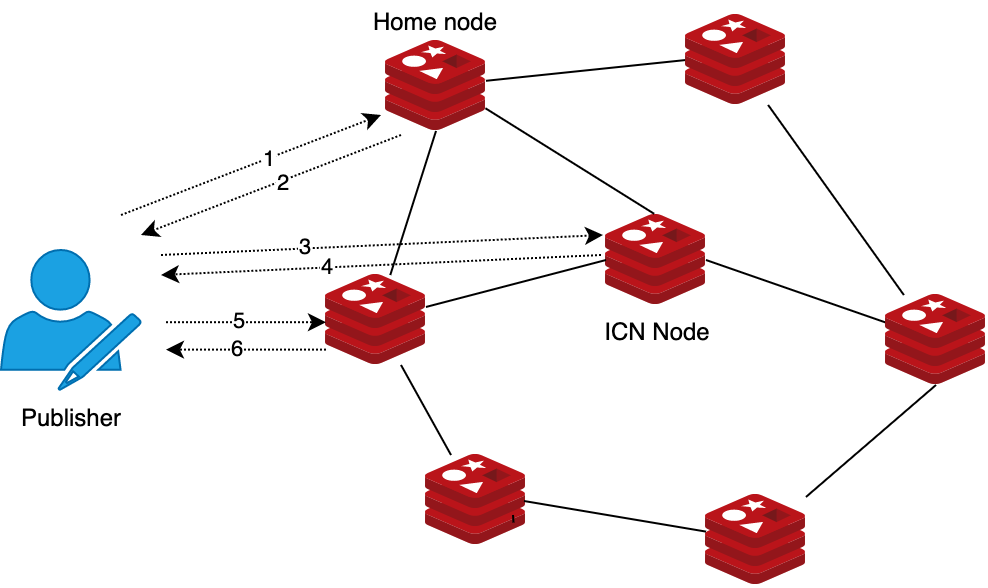
\includegraphics[width=\linewidth]{img/iterative-publications.png}
    \caption{Iterative publications of proof-of-time}
    \label{fig:iterative-publications}
\end{figure}

There are still some missing points that we need to solve. Although we can control infection dissemination speed, we do not have a mechanism to recover from malicious publications.  After a limited period of time the network should eventually notice the malicious publisher and reject the authentication. At the same time, an honest publisher who does not have time constraints can successfully infect the whole network––causing an epidemic and thus authenticating the content. 

We therefore need to add a node recovery mechanism. Once the node is infected, it should remain so for a limited period of time. After that time, it recovers, becoming healthy, i.e., distrusts the content. The period of time needs to be carefully designed so the nodes do not recover too fast because it would lead to the nodes getting infected slower than they are recovering. 

The requirement that the nodes be infected in succession is inconvenient. It would be much better if, following a limited succession of infections, another mechanism could infect the rest of the network.
For that, we can use an additional mechanism for inner infections. Each node gets infected not only by a publisher certificate, but also by the neighbor nodes. In this way, the publisher would be responsible just for starting the initial infection succession, which should embrace the whole network if it is long enough. 